% generated by scripts/pkl_to_latex.py
% source PKL : tscan_v1_L6_Ne6_U10_mode-uniform_nmin2_solver-gcg_full_restarts2_iter200_kmax4_tol1em09_t0.05to2_N20-d03538a42051.pkl
% scan type  : tscan
% state      : gs
% requires   : \usepackage{pgfplots} \pgfplotsset{compat=1.18}
% colours match the matplotlib PDF (tab10 cycle)
\definecolor{gmeC0}{HTML}{1F77B4}
\definecolor{gmeC1}{HTML}{FF7F0E}
\definecolor{gmeC2}{HTML}{2CA02C}
\definecolor{gmeC3}{HTML}{D62728}
\definecolor{gmeC4}{HTML}{9467BD}
\definecolor{gmeC5}{HTML}{8C564B}
\definecolor{gmeC6}{HTML}{E377C2}
\definecolor{gmeC7}{HTML}{17BECF}

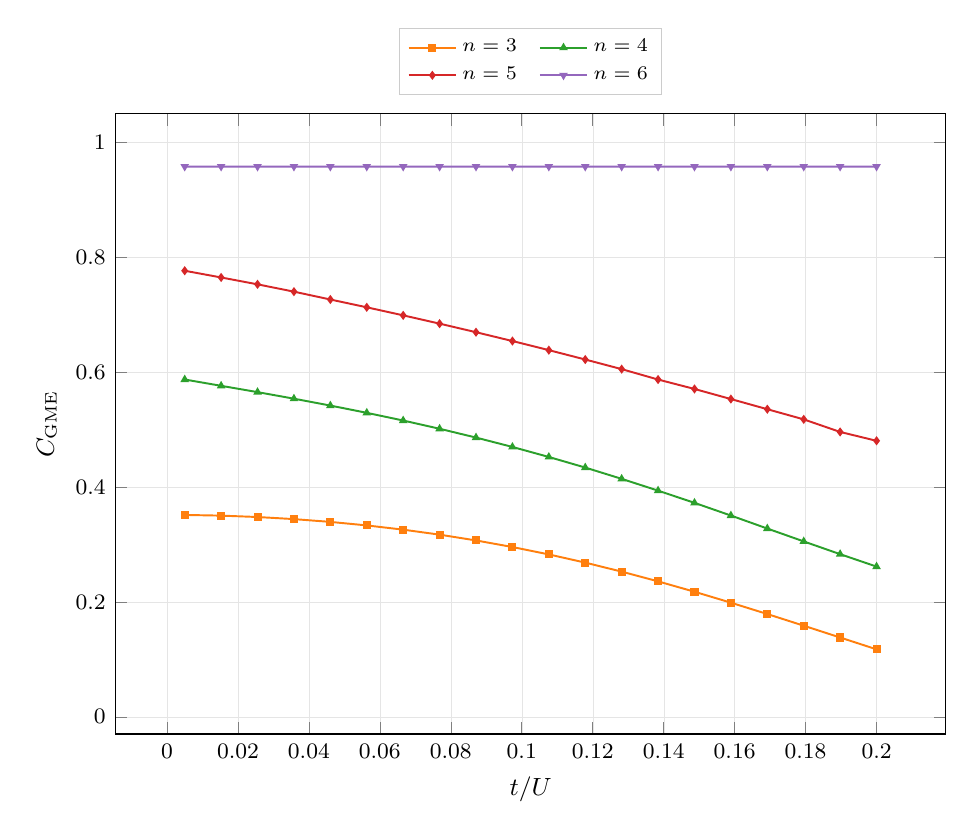
\begin{tikzpicture}
  \begin{axis}[
    width=\columnwidth,
    height=0.78\columnwidth,
    xlabel={$t/U$},
    ylabel={$C_{\mathrm{GME}}$},
    grid=both,
    grid style={line width=.1pt, draw=gray!20},
    tick label style={font=\footnotesize\rmfamily, /pgf/number format/fixed},
    label style={font=\small\rmfamily},
    scaled ticks=false,
    legend style={font=\scriptsize\rmfamily, draw=gray!40, at={(0.5,1.03)}, anchor=south, /tikz/every even column/.append style={column sep=6pt}},
    legend cell align={left},
    legend columns=2,
    ymin=-0.03,
    ymax=1.05,
  ]
    \addplot[color=gmeC1, mark=square*, mark size=1.1pt, line width=0.7pt] coordinates {
        (0.005,0.351546) (0.015263,0.350344) (0.025526,0.347925) (0.035789,0.344286)
        (0.046053,0.339418) (0.056316,0.333302) (0.066579,0.32591) (0.076842,0.317202)
        (0.087105,0.307136) (0.097368,0.295671) (0.107632,0.282786) (0.117895,0.268486)
        (0.128158,0.252817) (0.138421,0.235871) (0.148684,0.217785) (0.158947,0.198742)
        (0.169211,0.178956) (0.179474,0.158661) (0.189737,0.138096) (0.2,0.117491)
    };
    \addlegendentry{$n=3$}
    \addplot[color=gmeC2, mark=triangle*, mark size=1.1pt, line width=0.7pt] coordinates {
        (0.005,0.587379) (0.015263,0.576401) (0.025526,0.565424) (0.035789,0.553995)
        (0.046053,0.542009) (0.056316,0.52936) (0.066579,0.515967) (0.076842,0.501607)
        (0.087105,0.486284) (0.097368,0.46994) (0.107632,0.45249) (0.117895,0.434056)
        (0.128158,0.414382) (0.138421,0.393864) (0.148684,0.372586) (0.158947,0.350487)
        (0.169211,0.327862) (0.179474,0.305429) (0.189737,0.283226) (0.2,0.261585)
    };
    \addlegendentry{$n=4$}
    \addplot[color=gmeC3, mark=diamond*, mark size=1.1pt, line width=0.7pt] coordinates {
        (0.005,0.776773) (0.015263,0.765096) (0.025526,0.753123) (0.035789,0.740365)
        (0.046053,0.726703) (0.056316,0.713127) (0.066579,0.69912) (0.076842,0.684668)
        (0.087105,0.669756) (0.097368,0.654372) (0.107632,0.638517) (0.117895,0.622198)
        (0.128158,0.605452) (0.138421,0.58734) (0.148684,0.570911) (0.158947,0.553362)
        (0.169211,0.535655) (0.179474,0.517968) (0.189737,0.496061) (0.2,0.480641)
    };
    \addlegendentry{$n=5$}
    \addplot[color=gmeC4, mark=triangle*, mark size=1.1pt, mark options={rotate=180}, line width=0.7pt] coordinates {
        (0.005,0.958179) (0.015263,0.958179) (0.025526,0.958179) (0.035789,0.958179)
        (0.046053,0.958179) (0.056316,0.95818) (0.066579,0.95818) (0.076842,0.95818)
        (0.087105,0.958181) (0.097368,0.958182) (0.107632,0.958183) (0.117895,0.958185)
        (0.128158,0.958187) (0.138421,0.958189) (0.148684,0.958192) (0.158947,0.958195)
        (0.169211,0.958198) (0.179474,0.958201) (0.189737,0.958205) (0.2,0.958209)
    };
    \addlegendentry{$n=6$}
  \end{axis}
\end{tikzpicture}
